%第3章


\section{詳細設計}

オブジェクト間のメッセージのやりとりを時系列に沿って表現するためにシーケンス図を作成した.以下にICタグを用いた商品識別システムのシーケンス図,図\ref{sequence_ic}を載せる.

\begin{figure}[htbp]
\centering
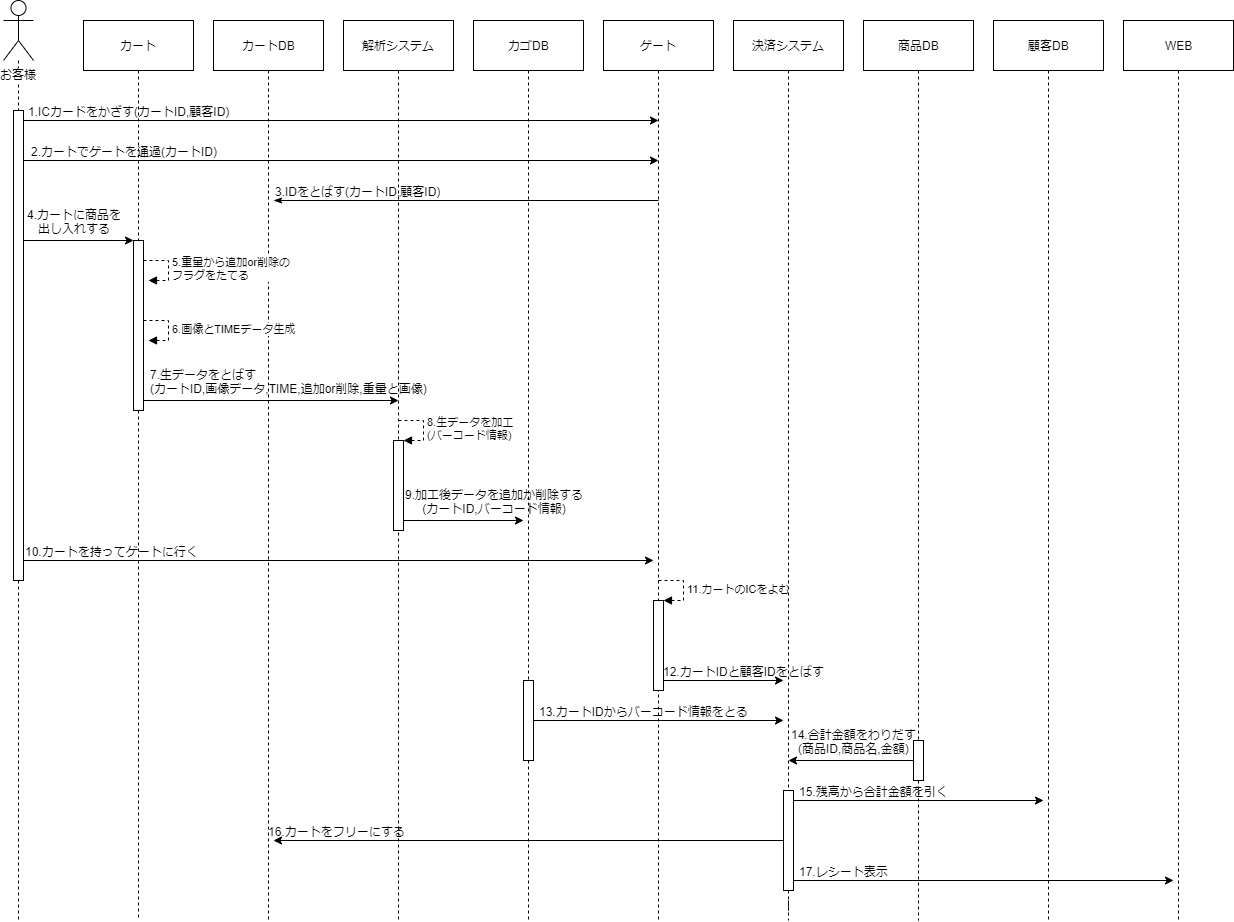
\includegraphics[width=15cm]{./picture/sequence_ic.eps}
\caption{ICタグを用いたシステムのシーケンス図}
\label{sequence_ic}
\end{figure}


以下の図\ref{sequence_qr}はQRコードを用いたシステムのシーケンス図である.


\begin{figure}[htbp]
\centering
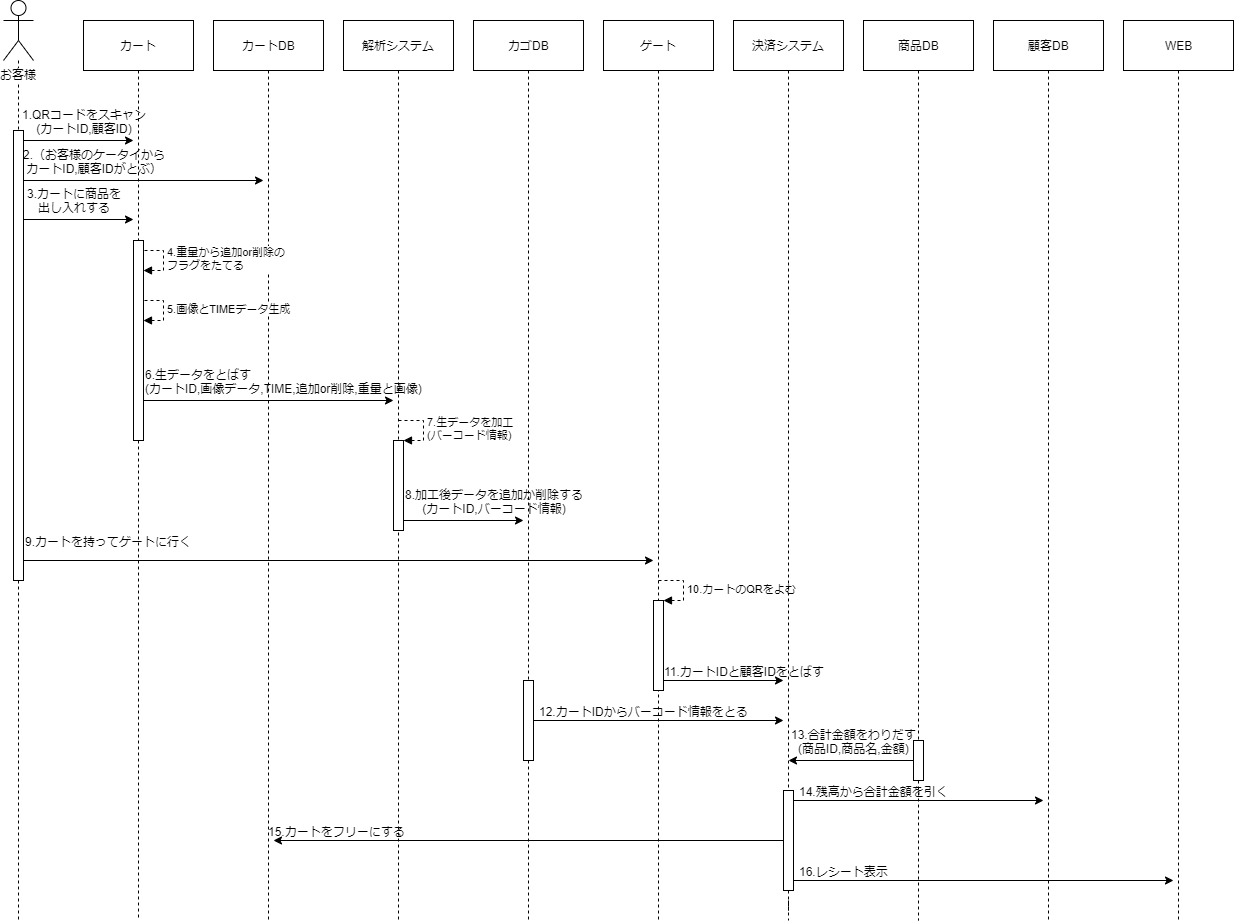
\includegraphics[width=15cm]{./picture/sequence_qr.eps}
\caption{QRコードを用いたシステムのシーケンス図}
\label{sequence_qr}
\end{figure}


上記図\ref{sequence_ic}と図\ref{sequence_qr}の違いはユーザ情報の登録の部分のみである.詳細設計まで行ったが,ICタグを用いたシステムとQRコードを用いたシステムの評価は3.1節から大きく変化しなかった.買い物と決済部分においては共通しているため,そのまま優先度の高いシステムである下記の図\ref{sequence}部分を実装する.



\begin{figure}[htbp]
\centering
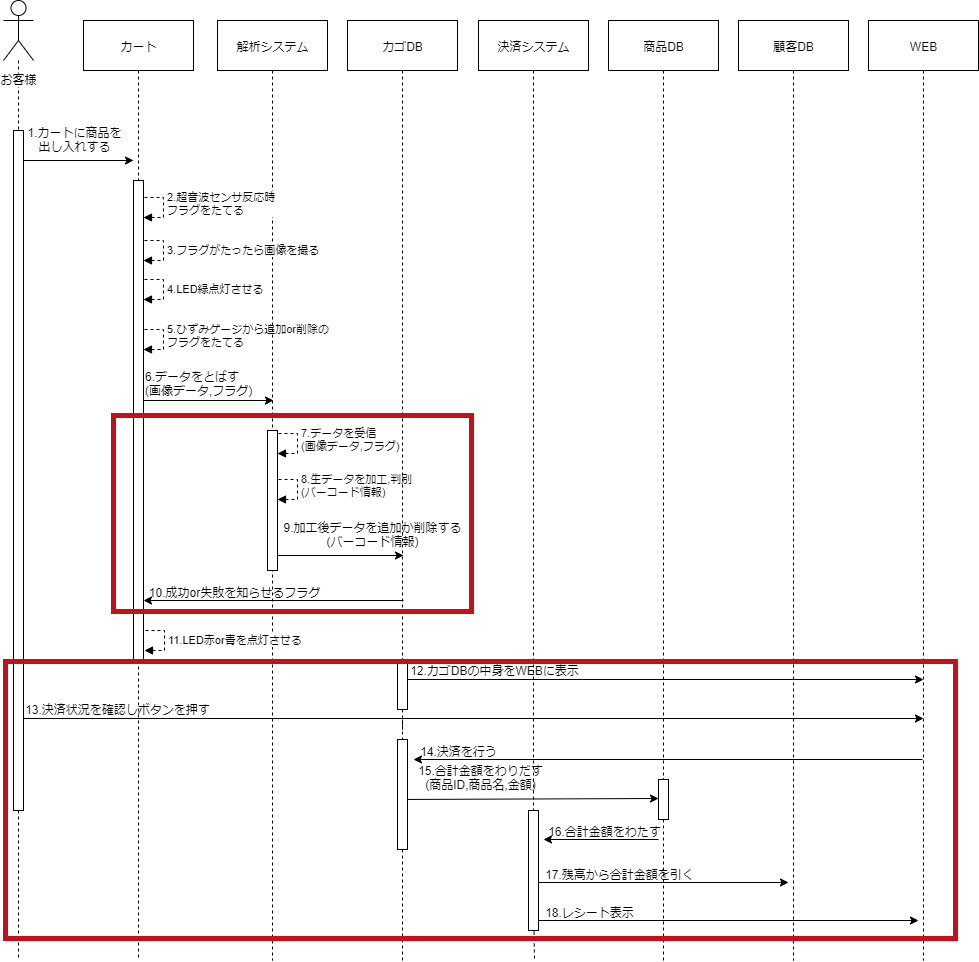
\includegraphics[width=15cm]{./picture/sequence.eps}
\caption{高優先度のシステムのシーケンス図}
\label{sequence}
\end{figure}


図\ref{sequence}において筆者の担当した部分はメッセージ2~6,10,11の部分である.各メッセージの詳細を下記に示す.


\begin{quote}
2. 超音波センサ反応時フラグをたてる

3. フラグが立ったら画像を撮る

4. LED緑点灯させる

5. ひずみゲージから追加もしくは削除のフラグをたてる

6. データを送信する(画像データ,追加か削除かを判定するフラグ)

10. 成功もしくは失敗を知らせるフラグを受信する

11. LED赤もしくは青を点灯させる
\end{quote}


%メッセージの説明